\documentclass[a4paper,10pt]{ltjsarticle}
\usepackage[top=22mm,bottom=23mm,left=25mm,right=25mm,footskip=10mm]{geometry}
\usepackage{amsmath,amssymb,booktabs,graphicx,xcolor}
\usepackage{hyperref}
\definecolor{linkink}{HTML}{215368}
\hypersetup{colorlinks=true,linkcolor=linkink,citecolor=linkink,urlcolor=linkink,
  pdftitle={行和・列和が高々2の3列二値行列の計数},
  pdfsubject={OEIS A401159 の3列公式の組合せ論的証明と Lean 4 による形式化},
  pdflang={ja-JP}}
\newcommand{\ident}[1]{\texttt{\detokenize{#1}}}
\newcommand{\rows}{[n]}
\newcommand{\entrylink}{https://github.com/oeis/oeisdata/blob/b460c2e8ffbef9a3aacf263819282712f0f30341/seq/A401/A401159.seq}
\setlength{\parindent}{1\zw}
\setlength{\abovedisplayskip}{7pt plus 2pt}
\setlength{\belowdisplayskip}{7pt plus 2pt}
\setlength{\emergencystretch}{1em}
\linespread{1.045}
% Both editions use the same theorem and the same seven published data points.
\newcommand{\threeColumnIdentities}{%
\begin{align}
 T(n,3) &= \left(1+n+\binom n2\right)^3-n^4+\binom n2 \label{eq:count}\\
        &= \frac{n^6+3n^5+n^4+13n^3+22n^2+8n+8}{8}. \label{eq:polynomial}
\end{align}%
}

\newcommand{\threeColumnValues}{%
\begin{tabular}{@{}lrrrrrrr@{}}
\toprule
$n$      &3&4&5&6&7&8&9\\
$T(n,3)$ &265&1\,081&3\,481&9\,367&22\,009&46\,585&90\,811\\
\bottomrule
\end{tabular}%
}

\raggedbottom

\begin{document}
\begin{center}
  {\LARGE\bfseries 行和・列和が高々2の3列二値行列の計数\par}
  \vspace{5pt}
  {\small 2026年11月25日\quad$\cdot$\quad\href{https://github.com/nktkt/math/blob/main/output/pdf/three-columns.pdf}{English edition}\par}
\end{center}
\smallskip

\noindent\textbf{要旨}\quad
各行・各列に1が高々2個ある $n\times3$ 二値行列を数える。
3列すべてが1の行に印を付け、同じ行列を二度数える場合を補正すると、
R.~J.~Mathar が OEIS A401159 に掲げた6次多項式が得られる。
この包除原理による証明を、任意の非負整数 $n$ について Lean~4 で形式化した。

\section{定義と主結果}
$\rows=\{1,\ldots,n\}$ とし、$[0]=\varnothing$ とする。
行と列に番号を付けた $n\times m$ 行列で、各成分が0または1、
各行および各列の和が2以下であるものの個数を $T(n,m)$ と書く。
Mathar は一般の行数・列数に対する漸化式と数表を与えた
\cite[第2節、表2]{mathar2014}。2026年には、次の等式~\eqref{eq:polynomial} を
3列の場合の予想として公表した \cite{oeis}。

\smallskip
\noindent\textbf{定理 1.}\quad 任意の非負整数 $n$ について
\threeColumnIdentities

\section{列の支持集合による証明}
第 $j$ 列で1が立つ行番号の集合を $S_j\subseteq\rows$ とする。
列の条件 $|S_j|\leq 2$ を満たす選び方は
$B=1+n+\binom n2$ 通りであり、列の条件だけを課した行列は $B^3$ 個ある。
このうち行の条件に違反するのは、3列すべてが1の行を含むものに限る。
そのような行の個数を $q=|S_1\cap S_2\cap S_3|$ とおく。各列の上限から $q\leq 2$ である。

まず、そのような行を一つ指定して $(A,i)$ の組を数える。
$i\in\rows$ を固定すると、各支持集合は $\{i\}$ または $\{i,a\}$（$a\ne i$）である。
したがって各列に $n$ 通りの選択肢があり、3列の選択は独立である。
$i$ の選び方を含めると、印を付けた組は $n\cdot n^3=n^4$ 個となる。

次に $q=2$ の行列を考える。該当する行を $i,k$ とすると、
すべての列で $S_j=\{i,k\}$ が強制される。逆に、どの2行を選んでも、
この指定で $q=2$ の行列がちょうど一つ得られる。その個数は $\binom n2$ である。

$B^3$ から $n^4$ を引くと、$q=1$ の行列は1回、$q=2$ の行列は2回引かれる。
後者を1回ずつ戻せば~\eqref{eq:count} が従う。
$\binom n2=n(n-1)/2$ を代入して展開すると~\eqref{eq:polynomial} を得る。
$n=0$ では両辺とも空の行列1個を数える。\hfill$\square$

\begin{center}
  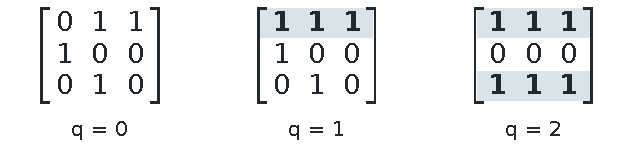
\includegraphics[width=.70\linewidth]{marked-rows.pdf}\par
  \smallskip
  {\small 図1\quad $n=3$ の例。網掛けは3成分すべてが1の行を示す。右の行列は印の選び方が二つある。}
\end{center}

\newpage
\section{2014年の数表からの導出}
式~\eqref{eq:polynomial} は、非零行の数に注目して次数を押さえると、
既存の数表からも導ける。$a_k$ を、行がすべて非零であることを追加条件とした
$k\times3$ の行列の個数とする。空の行列に対応して $a_0=1$ とおく。
3列の1の総数は高々6なので、非零行の数も高々6である。

非零行がちょうど $k$ 行の行列から零行を取り去り、残った行をもとの順序で並べると、
$a_k$ が数える行列が得られる。逆に、非零行の位置を $[n]$ の $k$ 元部分集合として選べば、
$a_k$ が数える行列から元の行列を一意に復元できる。よって
\begin{equation}
 T(n,3)=\sum_{k=0}^6 a_k\binom nk .\label{eq:basis}
\end{equation}
$n<k$ では $\binom nk=0$ とする。各 $\binom nk$ は $n$ に関する次数 $k$ の
有理係数多項式であるから、左辺も次数6以下の多項式である。

\begin{center}
{\small 表1\quad Mathar の表2にある3列の場合の値 \cite{mathar2014}。}\par
\smallskip
\threeColumnValues
\end{center}

式~\eqref{eq:polynomial} の右辺に $n=3,\ldots,9$ を代入すると表1の7値を得る。
次数6以下の多項式は相異なる7点での値から一意に定まるため、この照合と
式~\eqref{eq:basis} も証明を与える。OEIS の2026年11月25日閲覧版では
3列の公式に「Conjecture」と記載されている \cite{oeis}。
この公式の証明の歴史的な初出は未確認である。

\section{Lean 4 による形式化}
行列の型を \ident{Fin n} $\to$ \ident{Fin m} $\to$ \ident{Bool} とし、
各行・各列について、成分が真となる位置の集合の要素数が2以下であるという述語を定義した。
この述語を満たす行列の有限型の濃度が \ident{T n m} である。
有限集合の3組に移る際は、列の支持集合を取る操作と、それらの所属判定から
各成分を復元する操作が互いに逆であることを示した。

\ident{count_three_columns} は式~\eqref{eq:count} を自然数上の等式
\[
    T(n,3)+n^4=\left(1+n+\binom n2\right)^3+\binom n2
\]
として証明する。\ident{mathar_A401159_three_columns} はこれを有理数に移し、
二項係数を展開して OEIS と同じ係数の公式を得る。検証環境は Lean 4.29.1 である。
付属の \ident{PaperCheck.lean} は、紙面の多項式を行列の型から直接書き下して照合する。
固定した mathlib の版と再検証コマンドは
\href{https://github.com/nktkt/math/blob/main/README.ja.md}{日本語版の再現手順}に収録した。

\begin{thebibliography}{9}
\bibitem{mathar2014}
Richard J. Mathar, \emph{The number of binary $n\times m$ matrices with at most $k$
1's in each row or column}, 2014年11月23日。
\href{https://oeis.org/A247158/a247158.pdf}{論文 PDF}。
\bibitem{oeis}
Richard J. Mathar, \emph{OEIS A401159}, The On-Line Encyclopedia of Integer Sequences,
2026年11月18日、第9版。\href{https://oeis.org/A401159}{項目}、\href{\entrylink}{版を固定した原文}。
\end{thebibliography}
\end{document}
